\documentclass{article}
\usepackage{algpseudocodex}
\usepackage{algorithmicx}
\usepackage{enumitem}
\usepackage[boxed]{algorithm}
\usepackage{float}
\usepackage[utf8]{inputenc}
\usepackage{amsmath}
\usepackage{amssymb}
\usepackage{graphicx}
\usepackage{subfig}
\usepackage{tcolorbox}
\usepackage{listings}
\usepackage[left=20mm, right=20mm]{geometry}
\usepackage{enumitem}
\usepackage{amsthm}
\usepackage{algpseudocodex}
\usepackage{algorithmicx}
\usepackage[boxed]{algorithm}
\usepackage{hyperref}
\usepackage{tikz}
\usepackage{xcolor}
\usepackage{colortbl} % For coloring cells and text
\usepackage{amsmath}  % For mathematical symbols
\usetikzlibrary{shapes.geometric, arrows.meta, positioning, calc}

\newtheorem{theorem}{Theorem}
\newtheorem{lemma}{Lemma}
\newtheorem{corollary}{Corollary}[theorem]
\newtheorem{corollaryLemma}{Corollary}[lemma]
\newtheorem{prop}{Proposition}
\newtheorem{claim}{Claim}[theorem]

\definecolor{dupcolor}{RGB}{255,0,0} % Red
\definecolor{maxintcolor}{RGB}{165,42,42} % Brown
\definecolor{subsetsumcolor}{RGB}{0,0,255} % Blue

\lstset{showstringspaces=false,
        numbers=left, 
		numberstyle=\small}
\graphicspath{{}}

\algdef{SE}[CLASS]{Class}{EndClass}[1]{\textbf{Class} \textsc{#1}}{}
\algnewcommand{\AND}{\textbf{ and }}
\algnewcommand{\OR}{\textbf{ or }}
\algnewcommand{\Int}{\textbf{int }}
\algnewcommand{\Real}{\textbf{real }}

\title{COMP2123-Assignment 3}

\begin{document}
	\maketitle
	\section*{Notation Clarification}
	This section is to clarify the notations used throughout this assignment.
	
	\begin{center}
		\begin{tabular}{ c c }
			\([a:b]\) & The sequence \(a,\, a + 1, \ldots, \, b - 1\).\\
			\verb|int| & The data type representing integers.\\
			\verb|real| & The data type representing the real numbers.\\
			\verb|void| & Used to show that a function does not return anything.\\
			\verb|null| & The variable representing nothingness.\\
			\verb|bool| & The data type representing a boolean value which is either true or false.\\
		\end{tabular}
	\end{center} 

	\newpage \section*{Problem 1}

	\subsection*{a)}
	\begin{algorithm}[H]
		\caption{Wrong algorithm}
	\begin{algorithmic}[1]
		\Function{wrongAlgorithm}{M}
		\State \(M_{1}\), \(M_{2}\) \(\gets\) \(\emptyset\), \(\emptyset\) \Comment{Create two empty sets}
		\While{\(M\) contains some duplicate integer x}
			\State \(M \gets M \setminus \{x, x\}\) \Comment{Remove both instances of the duplicate integer x from the set M.}
			\State \(M_{1} \gets M_{1} \cup \{x\}\) \Comment{ Add one instance of the removed integer x to set M1.}
			\State \(M_{2} \gets M_{2} \cup \{x\}\) \Comment{Add the other instance of the removed integer x to set M2.}
		\EndWhile{}
		\While{\(M \neq \emptyset\)}
			\State \(x \gets \text{ largest integer in M }\)
			\State \(M \gets M \setminus \{x\}\) \Comment{Remove the largest integer x from set M}
			\If{there exist \(M^{'} \subseteq M \) s.t. x = sum of integers in \(M^{'}\)}
				\State \(M \gets M \setminus M^{'}\)  \Comment{Remove the subset M' from M.}
				\State \(M_{1} \gets M_{1} \cup \{x\}\) \Comment{Add the integer x to set M1}
				\State \(M_{2} \gets M_{2} \cup M^{'}\) \Comment{Add all integers in set M' to set M2.}
			\Else{}
				\State \Return{False}
			\EndIf{}
		\EndWhile{}
		\State \Return{True}
		\EndFunction{}
	\end{algorithmic}
	\end{algorithm}


	\begin{itemize}
		\item Let \textbf{Correct algorithm} is defined as an algorithm that consistently provides the correct answer for every possible input scenario of problem 1. Specifically, for any given set 
		M, this algorithm will return True if and only if 
		M can be partitioned into two subsets with equal sums, and False otherwise.
		\item The set M={1,1,7,3,4,2} is provided as input to the Correct Algorithm.  The Correct Algorithm returns True. The reasoning is illustrated in the diagram below:
	\end{itemize}
	
	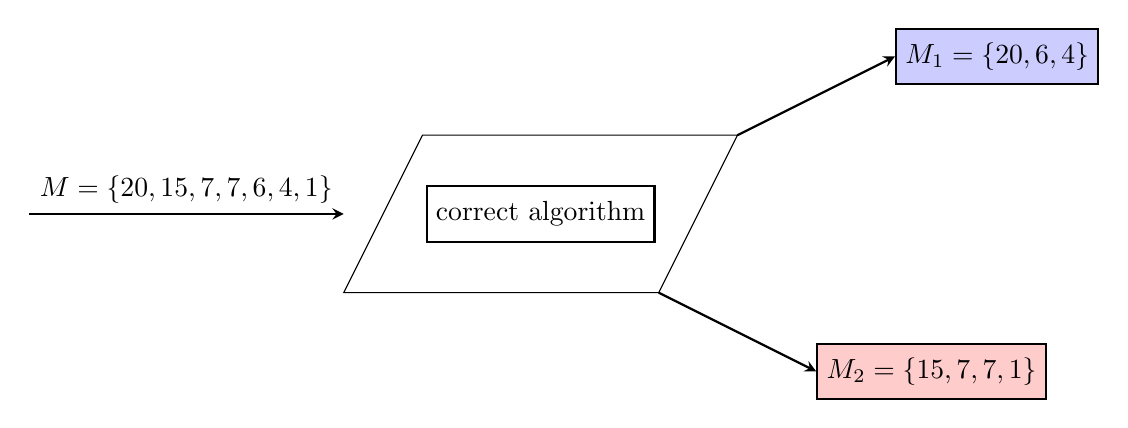
\begin{tikzpicture}
		% Define styles for bags and arrows
		\tikzstyle{bag} = [rectangle, thick, draw=black, text centered, minimum height=2em]
		\tikzstyle{arrow} = [thick,->,>=stealth]
		
		% Draw the main rectangle for M
		\node[bag] (m) at (2.5,1) {correct algorithm};
		\draw (0,0) -- (4,0) -- (5,2) -- (1,2) -- cycle;
		
		% Annotate the main rectangle
		\draw [arrow] (-4,1) -- node[above] {\(M = \{20, 15, 7, 7, 6, 4, 1\}\)} (0,1);
		
		% Draw and annotate arrows and rectangles for M1 and M2
		\draw [arrow] (5,2) -- (7,3) node[bag, fill=blue!20, anchor=west] {$M_1 = \{20, 6, 4\}$};
		\draw [arrow] (4,0) -- (6,-1) node[bag, fill=red!20, anchor=west] {$M_2 = \{15, 7, 7, 1\}$};
	
	\end{tikzpicture}

	As we can see in the graph, the sum of all elements in set \(M_{1} = \{20, 6, 4\}\) is \(20 + 6 + 4 = 30\).

	The sum of all elements in set \(M_{2} = \{15, 7, 7, 1\}\) is \(15 + 7 + 7 + 1 = 30\).

 	Therefore, both sets \(M_{1}\) and \(M_{2}\) have the same sum. \textbf{Correct algorithm} have to return True.

	\begin{enumerate}
		\item Testing the \textbf{WrongAlgorithm}
		\begin{itemize}
			\item The same set \(N = \{20, 15, 7, 7, 6, 4, 1\}\) is also input into a \textbf{WrongAlgorithm}
			\item Expected output: the wrong algorithm should return False.
			\item Conclusion from expected output: If the expected output is False, \textbf{WrongAlgorithm} does not correct in the case \(M = \{20, 15, 7, 7, 6, 4, 1\}\). Thus, \textbf{WrongAlgorithm} does not always return the correct answer and set \(M\) is a counterexample of \textbf{WrongAlgorithm}.
		\end{itemize}
		\item Tracking \textbf{WrongAlgorithm}
		\begin{table}[ht]
			\centering
			\caption{Description of Note}
			\label{note}
			\begin{tabular}{|c|c|}
			\hline
			\textbf{Note Color} & \textbf{Meaning} \\
			\hline
			\textcolor{dupcolor}{Red} & Duplicates element \\
			\hline
			\textcolor{maxintcolor}{Brown} & Largest integer \\
			\hline
			\textcolor{maxintcolor}{Brown} & A set containing the largest integer \\
			\hline
			\textcolor{subsetsumcolor}{Blue} & Subset with sum equal to the largest integer \\
			\hline
			\end{tabular}
			\end{table}
		\begin{table}[ht]
			\centering
			\caption{Tracking table}
			\label{tracking table}
			\begin{tabular}{|c|c|c|c|}
			\hline
			\rowcolor[HTML]{EFEFEF} 
			Line & \textbf{M} & \textbf{\textcolor{brown}{\(M_1\)}} & \textbf{\textcolor{blue}{\(M_2\)}} \\ \hline
			2 & \( \{20, 15, \textcolor{red}{7}, \textcolor{red}{7}, 6, 4, 1\} \) & \( \{\} \) & \( \{\} \) \\ \hline
			3 - 6 & \( \{\textcolor{brown}{20}, \textcolor{blue}{15}, 6, \textcolor{blue}{4}, \textcolor{blue}{1}\} \) & \( \{\textcolor{red}{7}\} \) & \( \{\textcolor{red}{7}\} \) \\ \hline
			7 - 15 & \( \{6\} \) & \( \{\textcolor{red}{7}, \textcolor{brown}{20}\} \) & \( \{\textcolor{red}{7},\textcolor{blue}{15} ,\textcolor{blue}{4}, \textcolor{blue}{1}\} \) \\ \hline
		\end{tabular}
		\end{table}
		\begin{itemize}
			\item In line 2 of the function, it creates two empty sets, which are \(M_{1}\) and \(M_{2}\) so in table \ref{tracking table}, we have the following sets.
			\item From line 3 to line 6 of \textbf{WrongAlgorithm}, use to find every duplicate integers then each of them are being seperated in each set. In \ref{tracking table}, we can see that set \(M\) has dupilicate integer is \textcolor{red}{7}, so \textcolor{red}{7} is being added one to each of \(M_1\) and \(M_2\). After the first while-loop, \(M = \{20, 15, 6, 4, 1\}\), \(M_1 = {7}\), \(M_2  = 7\).
			\item Because \(M \neq \emptyset\) so we run the second loop from line 7 - 15. In that loop, the function find the maximum integer in M, which equals to \textcolor{brown}{20}, after that function find the subset \textcolor{blue}{\(M^{'}\)} that have the sum of all elements that equals to maximum integer in \(M\). If we can not find, the function immediately return False. Otherwise, \(M_{1}\) will add largest elements in \(M\) and \(M_{2}\) equals to the \(M_2\) In \ref{tracking table} we can see that, \textcolor{brown}{20} is the largest integer in \(M\) and we can find a subset \textcolor{blue}{\(M^{'}\)} such that sum of all elements in 
			\textcolor{blue}{\(M^{'}\)} equals to \textcolor{brown}{20}, which is \textcolor{blue}{\(M^{'} = \{15, 4, 1\}\)}. Thus, after the first iteration in the second while loop, \(M = \{6\}\), \(M_1 = \{{\textcolor{red}{7}, \textcolor{brown}{20}}\}\) and \(M_{2} = \{\textcolor{red}{7}, \textcolor{blue}{15}, \textcolor{blue}{4}, \textcolor{blue}{1}\}\)
			\item After the first iteration, we can see that \(M = \{6\} \rightarrow M \neq \emptyset\), so the second will loop will continue to run one more time. At the second iteration, the largest integer in \(M\) now is 6. However, at this time, there do not have any \(M^{'} \subseteq M \) s.t. x = sum of integers in \(M^{'}\). Thus, the the conditional statement in line 10 will not run, it will run the else condition. Thus, the function return False and terminate.
		\end{itemize}
		\item Conclusion:
		\begin{itemize}
			\item As we can see, with the same input, \textbf{Correct Algorithm} return True, while \textbf{WrongAgorithm} return False. Thus, as what we say in Testing the \textbf{WrongAlgorithm}, if the ouput is False. \textbf{Wrong Algorithm} does not correct in the case \(M = \{20, 15, 7, 7, 6, 4, 1\}\). Thus, \textbf{WrongAlgorithm} does not always return the correct answer and set \(M\) is a counterexample of \textbf{WrongAlgorithm}
		\end{itemize}
	\end{enumerate}
	
	\subsection*{b)}
	\begin{algorithm}[H]
		\caption{Balancing algorithm}
	\begin{algorithmic}[1]
		\Function{balancingAlgorithm}{M}
		\State \(M_{1}\), \(M_{2}\) \(\gets\) \(\emptyset\), \(\emptyset\) \Comment{Create two empty sets}
		\State Sort M in non-increasing order
		\For{each integer x in M}
			\If{sum of integers in \(M_{1} \leq \) sum of integers in \(M_{2}\) }
				\State \(M_{1} \leftarrow M_{1} \cup \{x\}\)
			\Else{}
				\State \(M_{2} \leftarrow M_{2} \cup \{x\}\) 
			\EndIf{}
		\EndFor{}
		\State \Return{sum of integers in \(M_{1}\) = sum of integers in \(M_{2}\)}
		\EndFunction{}
	\end{algorithmic}
	\end{algorithm}

	\begin{enumerate}
		\item Testing \textbf{BalancingAlgorithm}
		\begin{itemize}
			\item The same set \(N = \{20, 15, 7, 7, 6, 4, 1\}\) is also input into a \textbf{BalancingAlgorithm}
			\item Expected output: the wrong algorithm should return False.
			\item Conclusion from expected output: If the expected output is False, \textbf{BalancingAlgorithm} does not correct in the case \(M = \{20, 15, 7, 7, 6, 4, 1\}\). Thus, \textbf{BalancingAlgorithm} does not always return the correct answer and set \(M\) is a counter-example of \textbf{BalancingAlgorithm}.
		\end{itemize}
		\item Tracking \textbf{BalancingAlgorithm}
		\item \begin{table}[ht]
			\centering
			\caption{Tracking balancing algorithm table}
			\label{balancing table}
			\begin{tabular}{|c|c|c|c|}
			\hline
			\rowcolor[HTML]{EFEFEF} 
			Line & \textbf{M} & \textbf{\(M_1\)} & \textbf{\(M_2\)} \\ \hline
			3 & \( \{\textcolor{red}{20}, 15, 7, 7, 6, 4, 1\} \) & \( \{\} \) & \( \{\} \) \\ \hline
			4 - 8 & \(\{20, \textcolor{red}{15}, 7, 7, 6, 4, 1\}\) & \(\{\textcolor{red}{20}\}\) & \(\{\}\)\\ \hline
			4 - 8 & \(\{20, 15, \textcolor{red}{7}, 7, 6, 4, 1\}\) & \(\{20\}\) & \(\{\textcolor{red}{15}\}\)\\ \hline
			4 - 8 & \(\{20, 15, 7, \textcolor{red}{7}, 6, 4, 1\}\) & \(\{20\}\) & \(\{15, \textcolor{red}{7}\}\)\\ \hline
			4 - 8 & \(\{20, 15, 7, 7, \textcolor{red}{6}, 4, 1\}\) & \(\{20, \textcolor{red}{7}\}\) & \(\{15, 7\}\)\\ \hline
			4 - 8 & \(\{20, 15, 7, 7, 6, \textcolor{red}{4}, 1\}\) & \(\{20, 7\}\) & \(\{15, 7, \textcolor{red}{6}\}\)\\ \hline
			4 - 8 & \(\{20, 15, 7, 7, 6, 4, \textcolor{red}{1}\}\) & \(\{20, 7, \textcolor{red}{4}\}\) & \(\{15, 7, 6\}\)\\ \hline
			4 - 8& \(\{\}\) & \(\{20, 7, 4\}\) & \(\{15, 7, 6, \textcolor{red}{1}\}\)\\ \hline
		\end{tabular}
		\end{table}
		\begin{itemize}
			\item In line 2, 3 of the function, it creates two empty sets, which are \(M_{1}\) and \(M_{2}\) and set \(M\) is sorted in non-increasing order  so in table \ref{balancing table}, we have the following sets.
			\item In the for-loop in line 4 to line 8, the function will iterate each element in M only once. I assume that the for-loop will iterate from left to right, which means from the largest to the smallest.
			\item In the first iteration, it will take \(\textcolor{red}{20}\) to set \(M_{1}\) because it will go through the if condition in line 5, which will calculate the sum of \(M_{1}\) and \(M_{2}\), which both equals to 0. Thus, \(\textcolor{red}{20}\) will come to set \(M_{1}\). 
			Similarity, it will continue to \textcolor{red}{15}. As we can see in table \ref{balancing table}, sum of all elements in \(M_{1}\) is larger than sum of all elements in \(M_{2}\). Thus, we will add \textcolor{red}{15} to \(M_{2}\). As a result, in the second iteration, \(M_{1} = \{20\}\) and \(M_{2} = \{15\}\).
			\item The for-loop will continue to iterate until it reachs every elements in \(M\) once time. At the last iteration, as we can see in \ref{balancing table}, \(M_{1} = \{20, 7, 4\}\) have the sum is 31 and \(M_{2} = \{15, 7, 6\}\) have the sum is 28. Thus, \textcolor{red}{1} have to be in set \(M_{2}\) (because sum of all elements in \(M_{1}\)) is larger than sum of all elements in \(M_{2}\). After the iteration
			we have \(M_{1} = \{20, 7, 4\}\) and \(M_{2} = \{15, 7, 6, 1\}\) so the sum of all elements in \(M_1\) is 31 and sum of all elements in \(M_{2}\) is 29. So the \textbf{Balancing Algorithm} will return False in line 9.
		\end{itemize}
		\item Conclusion
		\begin{itemize}
			\item As we can see, with the same input, \textbf{Correct Algorithm} return True, while \textbf{Balancing Algorithm} return False. Thus, as what we say in Testing of \textbf{Balancing Algorithm}, if the output is False, the \textbf{Balancing Algorithm} does not correct in the case \(M = \{20, 15, 7, 7, 6, 4, 1\}\). Thus, the \textbf{Balancing Algorithm} does not always return the correct answer and set M is a counter example of \textbf{Balancing Algorithm}.
		\end{itemize}
	\end{enumerate}

	\newpage \section*{Problem 2}
	\subsection*{a)}
	This is the following methods of doubly-linked list we have to use.
	\begin{itemize}
		\item \verb|Node first()|: Return the first \textbf{Node}(head) of that doubly-linked list. \(O(1)\)
		\item \verb|Node last()|: Return the last \textbf{Node}(tail) of that doubly-linked list. \(O(1)\)
		\item \verb|void remove(Node p)|: Remove the Node p out of that doubly-linked list. This method also update the head and tail of that doubly-linked list after removing Node p. \(O(1)\)
		\item \verb|bool is_empty()|: indicates wheather no elements are stored. \(O(1)\)
	\end{itemize}
	To implement doubly-linked list we need to have Node object with some attributes such as \textbf{next}, \textbf{prev} and \textbf{value}.

	\begin{algorithm}[H]
		\caption{Class Node}
		\begin{algorithmic}
			\Class{Node}
				\State \textbf{int} value \Comment{The value store in the Node}
				\State \textbf{Node} next \Comment{The reference to the next node, null if it is the end node}
				\State \textbf{Node} prev \Comment{The reference to the previous node, null if it is the head of that doubly-linked list}
			\EndClass
		\end{algorithmic}
	\end{algorithm}

	Because \textbf{REMOVE-MIN} and \textbf{REMOVE-MAX} is on the union of the lists, we have to add more attribute to class Node, which names is \textbf{belong}. This attribute will return the doubly-linked list that contains that Node. This attribute will help us know where the Node is in. 

	Thus, the Node class below is the update version.

	\begin{algorithm}[H]
		\caption{Class Node}
		\begin{algorithmic}
			\Class{Node}
				\State \textbf{int} value \Comment{The value store in the Node}
				\State \textbf{Node} next \Comment{The reference to the next node, null if it is the end node}
				\State \textbf{Node} prev \Comment{The reference to the previous node, null if it is the head of that doubly-linked list}
				\State \textbf{Doubly\_ll} belong \Comment{The reference to the doubly-linked list that the Node is in}
			\EndClass
		\end{algorithmic}
	\end{algorithm}

	\begin{itemize}
		\item Now, I will build a min-heap and max-heap with size k. To build a min-heap and a max-heap, I implement heap-in-array implementation, I need to have two array of length k, one for max-heap and another one for min-heap.


		\item With k non-empty sorted doubly-linked list, I assume that all of them is in non-increasing order. Thus, the head of that doubly-linked list will have the largest value in that doubly-linked list, and the tail of that doubly-linked list will be the smallest value of that doubly-linked list.
		\begin{itemize}
			\item \textbf{min\_array}: This array uses to build min-heap. Thus, every element in this array will be the last Node(tail) of k sorted doubly-linked list.
			\item \textbf{max\_array}: This array uses to build max-heap. Thus,every element in this array will be the first Node(head) of k sorted doubly-linked list.
		\end{itemize}
		
		\item To put k \textbf{Node} in array, I will have the following pseudocode. This pseudocode will assume k doubly-linked list will be stored in an array with k elements and each element in that array is doubly-linked list object. I call that array is \textbf{collections}.


		\begin{algorithm}[H]
			\caption{Add k Node in array}
		\begin{algorithmic}[1]
			\Function{storingNode}{\textbf{Array} min\_array, \textbf{Array} collections}
			\State index \(\leftarrow\) 0
			\For{each doubly-linked list object k in collections}
				\State array.add(index, k.last())
				\State index \(\gets\) index + 1
			\EndFor{}
			\State \Return{\textbf{min\_array}}
			\EndFunction{}
		\end{algorithmic}
		\end{algorithm}

		\item I always add Node object at the end of an array so add function do not need to shifting forward. Thus, add function always run in \(O(1)\), with k doubly-linked list object, \textbf{storingNode} will run in \(O(k)\) time.
		\item To make \textbf{max\_array} store Node, it will be similar to \textbf{storingNode} with a few changes in the parameter in line 1, change to max\_array and instead of using \(k.last()\) in line 4, it has to be \(k.first()\)
		\item After having two arrays, now we will use that to implement heap-in-array with some important properties.
		\begin{itemize}
			\item Special Node
			\begin{itemize}
				\item root is at 0
				\item last node is at n - 1
			\end{itemize}
			\item For the node at index i:
			\begin{itemize}
				\item The left child is at index \(2i + 1\)
				\item The right child is at index \(2i + 2\)
				\item Parent is at index \( \lfloor (i - 1) / 2 \rfloor\)
			\end{itemize}
		\end{itemize}
		\item This pseudocodes below is how I build max-heap
		\begin{itemize}
			\item To build max-heap, we need a function calls \textbf{heapify}
			\begin{algorithm}[H]
				\caption{Heapify function}
			\begin{algorithmic}[1]
				\Function{heapify}{\textbf{int} index,\textbf{Array} max\_array}
				\State length \(\gets\) length of max\_array
				\State \(n \gets\) \( \lfloor (length - 1) / 2 \rfloor\) \Comment{n is the last index that have child}
				\If{index \(>\) n}
					\State \Return{\textbf{null}} \Comment{Heapify function just take index that have child as a parameter, if not, we will return. This is the base case}
				\EndIf{}
				\State left\_child \(\leftarrow 2 \times \text{index} + 1\) \Comment{location of left child of index}
				\State right\_child\_2 \(\leftarrow 2 \times \text{index} + 2\) \Comment{location of right child of index}
				\State largest \(\gets\) index
				\If{left\_child \(<\) length \textbf{and} max\_array[left\_child].value \(>\)  max\_array[index].value}
					\State largest \(\gets\) left\_child
				\EndIf{}

				\If{right\_child \(<\) length \textbf{and} max\_array[right\_child].value \(>\)  max\_array[largest].value}
					\State largest \(\gets\) right\_child
				\EndIf{}

				\If{largest \(\neq\) index}
					\State node\_temporary \(\gets max\_array[index]\)
					\State max\_array[index] \(\gets  max\_array[largest]\)
					\State  max\_array[largest] \(\gets node\_temporary\)
					\State heapify(largest, max\_array) \Comment{After finish swaping, we continue to heapify at index}	
				\EndIf{}
				\EndFunction{}
			\end{algorithmic}
			\end{algorithm}
			\item Then I will use heapify to build a heap with function calls \textbf{build\_heap}
			\begin{algorithm}[H]
				\caption{Build heap}
			\begin{algorithmic}[1]
				\Function{build\_heap}{\textbf{Array} max\_array}
				\State i \(\gets\) \(\lfloor (\text{length of max\_array} - 1) / 2 \rfloor\) \Comment{We will start heapify from the last index that have child to root index, which is 0}
				\While{\(i >= 0\)} 
				\State heapify(i, max\_array)
				\State i \(\gets\) i - 1
				\EndWhile{}
				\State \Return{\textbf{max\_array}}
				\EndFunction{}
			\end{algorithmic}
			\end{algorithm}
		\end{itemize}
		\item Build min-heap is similar to build max-heap with some changes of the function heapify.
		\begin{itemize}
			\item The parameter is not max\_array, it will become min\_array
			\item Instead of marking \textbf{largest} equals to the child index that have the Node contains largest value, We will mark the \textbf{largest}(We can change it to \textbf{smallest}) equals to the child index that have the Node contains smallest value. (Change \(>\) to \(<\) in line 9 and line 11)
		\end{itemize}
		\item After I finish build heap. Now we have some properties in two arrays \textbf{min\_array} and \textbf{max\_array}.
		\begin{itemize}
			\item The first index in \textbf{min\_array} contains the Node that have the smallest value in \textbf{min\_array}, which means that Node that have smallest value comparing to every Node in k doubly-linked list. This is mainly because we store every Node that have smallest value in each doubly-linked list in \textbf{min\_array}.
			\item Similar to first index in \textbf{max\_array} contains the Node that have the largest value in \textbf{max\_array}, and that Node also have largest value comparing to every Node in k doubly-linked list.
		\end{itemize}
		\item Before implements \textbf{REMOVE-MIN} and \textbf{REMOVE-MAX}, I need to create two more functions, which name are \textbf{removeTop(Array array)} and \textbf{insert(Node node, Array array)}.
		\begin{itemize}
			\item The reason I need two create two more functions is that, I need to take the root of the heap out when calling \textbf{REMOVE-MIN} and \textbf{REMOVE-MAX} functions. Then, I will remove that node at that doubly linked list, before insert the tail of that doubly linked list back to the heap. 
		\end{itemize}
		\item \verb|Node removeTop(Array array)|: Return the root of the heap
		\item \verb|void insert(Node node, Array array)|: insert Node node into a heap.
		
		\begin{algorithm}[H]
			\caption{Remove root in heap}
		\begin{algorithmic}[1]
			\Function{removeTop}{\textbf{Array} array}
			\State node \(\gets\) array[0] \Comment{the node will be removed}
			\State array[0] \(\gets\) array[length of array - 1] \Comment{Replace the root with the last element}
			\State array\(\gets\) array[0 : length of array - 1] 
			\State heapify(0, array) \Comment{use heapify function at root of the heap, this function can be a version of heapify for min-heap and max-heap}
			\State \Return{node}
			\EndFunction{}
		\end{algorithmic}
		\end{algorithm}


		\begin{algorithm}[H]
			\caption{Insert Node node into heap}
		\begin{algorithmic}[1]
			\Function{insert}{\textbf{Node} node,\textbf{Array} array}
			\State i \(\gets\) the length of array \Comment{first i will equals to array length}
			\State array.add(i, node) \Comment{Assume array will not be full capacity}
			\While{array[\(\lfloor (i - 1) / 2 \rfloor\)].value \(<\) array[i].value} \Comment{Fix the heap properties if it is violated}
				\If{i = 0}
					\State \verb|break|
				\EndIf{}
				\State temporary\_node \(\gets\) array[\(\lfloor (i - 1) / 2 \rfloor\)]
				\State array[\(\lfloor (i - 1) / 2 \rfloor\)] \(\gets\) array[i]
				\State array[i] \(\gets\) temporary\_node
			\EndWhile{}
			\EndFunction{}
		\end{algorithmic}
		\end{algorithm}
		\item From every properties I have mentioned before and all function I have just built, we can use them to implements \textbf{REMOVE-MIN} and \textbf{REMOVE-MAX} function.
		\begin{algorithm}[H]
			\caption{REMOVE MAX}
		\begin{algorithmic}[1]
			\Function{REMOVE\_MAX}{\textbf{Array} max\_array}
				\State node \(\gets\) removeTop(max\_array) \Comment{Remove the root of the heap and node will be the node at the root of the heap} 
				\State node.belong.remove(node) \Comment{Find that doubly-linked list that contains that node then remove that node using remove methods}
				\State insert(node.belong.first(), max\_array) \Comment{After remove that doubly-linked list, then we insert the newest head of that doubly-linked list into max-heap}
			\EndFunction{}
		\end{algorithmic}
		\end{algorithm}



		\begin{algorithm}[H]
			\caption{REMOVE MIN}
		\begin{algorithmic}[1]
			\Function{REMOVE\_MIN}{\textbf{Array} min\_array}
				\State node \(\gets\) removeTop(min\_array) \Comment{Remove the root of the heap and node will be the node at the root of the heap} 
				\State node.belong.remove(node) \Comment{Find that doubly-linked list that contains that node then remove that node using remove methods}
				\State insert(node.belong.last(), min\_array) \Comment{After remove that doubly-linked list, then we insert the newest head of that doubly-linked list into max-heap}
			\EndFunction{}
		\end{algorithmic}
		\end{algorithm}


		\item Overview data structure.
		\begin{itemize}
			\item First I will, build a Max-heap and Min-heap with every elements in Max-heap is the head of k doubly-linked list and every elements in Min-heap is the tail of k doubly-linked list.
			\item After finishing building heaps, in \textbf{REMOVE-MIN} and \textbf{REMOVE-MAX}, I calls \textbf{removeTop} to remove the node at the root of each heap.
			\item Then, I will remove that node at the doubly-linked list that contains that node.
			\item Finally, I call \textbf{insert} function to insert tail of that-doubly linked list for min heap and head of that doubly-linked list for max heap into each heap  
		\end{itemize}
	\end{itemize}

	\subsection*{b)}
	\begin{itemize}
		\item As I mentioned before, root of Min-heap and Max-heap always holds the node that have maximum value and minimum value of union of thest lists. The reason for that is because all of the doubly-linked list is being sorted so in min\_array, we store all node that have smallest value in each doubly-linked list, and in max\_array, we store all node that have largest value in each doubly-linked list. At the same time, root of Min-heap is the smallest value in min\_array and root of Max-heap is the largest value in max\_array. Thus, root of Min-heap is the node that have smallest value and root of Max-heap is the node that have largest value.
		\item After I remove the root of the heap and that in that doubly-linked list that have that node, then I will insert newest head or tail of that doubly-linked list. Thus, we need  to insert the Node that have the second maxima value in that doubly-linked list, so we insert to that heap. Following this rountine ensures the heap's order is consistently. 
		\item \textbf{Argue the Correctness (Proving the correctness using loop invariant)}
		\begin{itemize}
			\item \textbf{Invariant}: Because my min\_array and max\_array after being built by using \textbf{BUILD\_HEAP} function always contains Nodes with the smallest elements and largest value in each array. All of these elements locate at the head of doubly-linked lists(max) and tail of doubly-linked lists(min), the root of min-heap(first Node in min\_array) and max-heap(first Node in max\_array) are always be the Nodes with smallest value and largest value in all k doubly-linked lists. This is true because every our doubly-linked lists is being sorted(non-increasing order) and the property of min-heap and max-heap are the root always be the Node that minimum and maximum value.
			\item \textbf{Initialization}: Before calling \textbf{REMOVE-MIN} or \textbf{REMOVE-MAX}, the Node with smallest value is at the root of the heap(First element in array). When I call \textbf{REMOVE-MIN} and \textbf{REMOVE-MAX}, first it will remove the root of the heap by using \textbf{REMOVE-TOP} function. This function remove by swaping root Node and last Node in heap(last element in an array), then using \textbf{HEAPIFY} function at the root of the heap to keep the property of the heap always True(The parent always larger than their children(max heap), the parent always smaller than their children(min heap)). Thus, after using removing root Node out of heap, the invariant still holds. After that, I have to insert the second smallest or second largest into heap. Because we have to keep the size of heap constant. Thus, I calls \textbf{insert} to insert next Node to heap and it also maintains the heap property because of while loop in insert function to fix the heap properties if it is violated.
			\item \textbf{Termination}: When \textbf{REMOVE-MIN} or \textbf{REMOVE-MAX} completes, the Node with smallest or largest value is being removed, then it also insert the another Node the prepare for the next call. As a result, the invariant always keep that at every point of the operation, the root of the heap always the Node that we will remove first.
		\end{itemize}
	\end{itemize}

	\subsection*{c)}
	\begin{enumerate}
		\item Running time of \textbf{HEAPIFY} function:
		\begin{enumerate}
			\item Running time:
			\begin{itemize}
				\item The comparision operation at line 9 and 11 take constant time
				\item The swap operaton betweeen line 14 and 16 take constant time
				\item The recursive call in line 17 in worst case, the element at index may need to be moved down the height of the heap. However, a heap is a complete tree, its height is \(O(log(k))\). Thus, in the worst cast the function will move an  down from the root to leaf node, making a single recursive call at each level of the tree. Therefore, the running time of the \textbf{HEAPIFY} is \(O(log(k))\)
			\end{itemize}
		\end{enumerate}
		\item Running time of \textbf{REMOVE\_TOP} function:
		\begin{enumerate}
			\item Running time:
			\begin{itemize}
				\item Line 2 and 3: Storing the root's value and replacing it with the last element are both constant time operation
				\item Adjusting the size of the heap is also constant time
				\item Running time of \textbf{HEAPIFY} function is \(O(log(k))\)
				\item Therefore the running time of \textbf{REMOVE\_TOP} function is \(O(log(k))\)
			\end{itemize}
		\end{enumerate}
		\item Running time of \textbf{INSERT} function:
		\begin{enumerate}
			\item Running time:
			\begin{itemize}
				\item Line 2: Assigning the length of the heap to i is a constant time.
				\item Line 3: Adding the new node to the end of the array is also constant time under the assumption that the heap is not at full capacity and does not need to resize. \(O(1)\)
				\item Line 4 - 9: In the worst case, the new node needs to be compared and possibly swapped with each of its ancestors until it reach the correct position in the heap. Since a heap is a completed tree, the height of the heap and therefore the number of ancestors, is \(log(k)\)
				\item Therefore, in the worst case, the new node will be compared and swapped with each of its ancestors, resulting in a running time of \(O(logk)\)
			\end{itemize}
		\end{enumerate}
		\item Running time of initialising data structure.
		\begin{enumerate}
			\item Running time:
			\begin{itemize}
				\item  My data strucuture is heap-in-array implementation, so first I need to have two array with size of k, one is min\_array and another one is max\_array. To optimise the running time of import k Node(head) to max\_array and k Node(tail) to min\_array, I create two array with size k first. After that, I will create a varable to keep track the place to add in array in O(1), which is the last index of an array. Thus with k time add, the complexity is \(O(k)\)
				\item After I have an array, then I will call \textbf{BUILD-HEAP} function to make a heap from arrays. This function will scan every Node that have child in heap(from 0 to \(\lfloor (\text{length of array} - 1) / 2 \rfloor\)). At each parents Node, I call \textbf{HEAPIFY} at that index. According the lecture, \textbf{a heap on n keys can be constructed in \(O(n)\) time}. Thus, with k Node in array, I can construct a min-heap and max-heap in \(O(k)\)
			\end{itemize}
			\item Conclusion: Thus, the total time of initialising is \(O(k)\) time
		\end{enumerate}
		\item Running time of REMOVE-MIN and REMOVE-MAX
		\item \begin{enumerate}
			\item Running time:
			\begin{itemize}
				\item Line 2: The \textbf{REMOVE\_TOP} has running time of \(O(log(k))\)
				\item The removal operation on a doubly-linked list is generally \(O(1)\)
				\item Line 4: The \textbf{INSERT} has running time of \(O(log(k))\)
			\end{itemize}
			\item Conclusion: Thus, the running time of REMOVE-MIN and REMOVE-MAX \(O(log(k))\) time
		\end{enumerate}
	\end{enumerate}


	\newpage \section*{Problem 3}


	To support the operations in Problem 3, I will use the following data structure.
	\begin{itemize}
		\item \verb|AVL Binary search tree for main dish|: This binary search tree use to store every main dishes in the restaurant. This data structure will help us to implement \textbf{removeMainDish} function and \textbf{AddNewMainDish} function. To support functions, this binary search tree have to search by the name of the dish. Thus, this binary search tree will use the name(\verb|String|) as a key to search using(lexicographic order). I call this tree is \textbf{MainDishTree}
		\item \verb|AVL Binary search tree for a side dish|: This binary search tree use to store every side dishes in the restaurant. This data structure will help us to implement \textbf{removeSideDish} function and \textbf{AddNewSideDish} function. To support functions, this binary search tree have to search by the name of the dish. Thus, this binary search tree will use the name(\verb|String|) as a key to search using(lexicographic order). I call this tree is \textbf{SideDishTree}
		\item \verb|Three arrays with size 16|: The first two arrays use to store the distribution of price of the main dish and side dish, calling \textbf{Main\_array} and \textbf{Side\_array}, which means each entry store how many dish with that price. For example, \textbf{Main\_array[5] = 6} means we have 6 main dish with price 5\$. The price will be the index(price is a positive integer) of Main\_array and the value stores at Main\_array at that index will be the number of Main dish 
		The last array is \verb|prefixDish|, this array will have the size 16, this array use to calculate prefix sum for \textbf(Side\_array[i]), which means \textbf{prefixDish[i]} is equals to the sum of \textbf{prefixDish[i - 1]} with \textbf{Side\_array[i]}
	\end{itemize}

	The reason we have to build AVL tree instead of normal binary search tree is because, in the worst case height(h) of the binary search tree equals to the number of node in the trees(n) so the running time of insertion and deletion in the worst case is \(O(n)\). Thus we need to use AVL tree to storing with the height of AVL tree always \(O(log(n))\). This can be proved by using induction(Slide 45 at week binary search tree)
	
	\begin{itemize}
		\item Let N(h) be the minimum number of keys of an AVL tree of height h
		\item We easily see that N(1) = 1 and N(2) = 2(base case)
		\item Clearly \(N(h) > N(h - 1)\) for any \(h \geq 2\)
		\item For \(h > 2\), the smallest AVL tree of height h contains the root node, one AVl subtree of height \(h - 1\) and anotehr of height at least \(h - 2\)
		\[N(h) \geq 1 + N(h - 1) + N(h - 2) \geq 2N(h - 2)\]
		\item By induction we can show that for h even
		\[N(h) \geq 2^{\frac{h}{2}}\]
		\item Taking logarithm: \(h < 2 log(N(h))\)
		\item Thus the height of an AVL tree is \(O(logn)\)
	\end{itemize}

	In slide 59, week 4, the lecture said that
	\begin{itemize}
		\item The data structure use O(n) space
		\item Height of the tree is \(O(log(n))\)
		\item Searching takes \(O(log(n))\)
		\item insertion takes \(O(log(n))\)
		\item Removal takes \(O(log(n))\)
	\end{itemize}

	AddNewMainDish(\textbf{String} name, \textbf{int} price) and AddNewSideDish(\textbf{String} name, \textbf{int} price) can be implemented as below.
	\begin{itemize}
		\item Using name as a key for AVL tree using lexiographic order. This key(String) is then used as a key to to insert the element into a AVl tree, aloowing for organized and efficient access based on the index. Additionally, the system updated the distribution of prices by incrementing the count in \textbf{Main\_array[price]} or \textbf{Side\_array[price]}. If the price is larger than 15\$, we will skip the step updating the distribution of prices.
		\item Remember that I use insert function in AVl tree so it always keep the tree balance and another thing to note that I do not encrypt key String name to integer to compare. I use lexicographic order to compare String with String immediately. Lexicographic order comparison involves sorting elements based on their sequence, similar to how words are arranged in a dictionary. Each element is compared character by character from left to right, with the first differing character determining their order. This method is used not only for words but also for sequences of numbers or other sortable data.
	\end{itemize}
	removeMainDish(\textbf{String} name) and removeSideDish(\textbf{String} name) can be implemented as below
	\begin{itemize}
		\item Because I use name as a key for AVl tree when I insert Node into AVl tree, so when I want to delete some Node out of the tree, I can use \textbf{String} name to delete them. Thus, I use delete function of AVl tree with key is name to delete that Node out of the tree. After that, I have to update the distribution of the price by decrementing the value of Main\_array[price] or Side\_array[price] by 1 with price is the price of the Node we deleted. If the price of the Node being deleted is more than 15\$, I will skip the step of updating distribution of price array
	\end{itemize}

	countCombination()
	\begin{itemize}
		\item Now, I have two array for main dish and side dish with the index is the price of the dish with the value of that index is the number of main dish or side dish at that price. Now the third array calls \textbf{computing} will have size of 16 to do preprocessing.
		\[computing[i] = 0 \text{ if i = 0}\]
		\[computing[i] = computing[i - 1] + Side\_array[i -1] \text{if i larger than 0}\]
		\item Iterate over every pair \(0 \leq i \leq j < 16\)
		\item Use this algorithm, I call i is the index of computing. Thus computing[i] equals to number of dish that have price below (i - 1)\$.
		\item After having this array, I will iterate every element in main\_arraym, I have the variable calls \textbf{result}, each time I iterate to each element in main\_array.
		\[result = result + main\_array[i] + computing[16 - i + 1]\]
	\end{itemize}
	
	This one is the pseudocode.

	\begin{algorithm}[H]
		\caption{countCombination}
	\begin{algorithmic}[1]
		\Function{countCombination}{}
		\State i \(\leftarrow\) 0 
		\While {i to 15}
			\If{i = 0}
				\State computing[i] = 0
			\Else{}
				\State computing[i] = computing[i - 1] + side\_array[i - 1]
			\EndIf{}
			\State i \(\leftarrow\) i + 1
		\EndWhile{}
		\State i \(\leftarrow\) 0 
		\State result \(\gets\) 0
		\While{i to 15}
			\State result \(\gets\) result + main\_dish[i] \(\times\) computing[15 - i + 1]
		\EndWhile{}
		\State \Return{\textbf{result}}
		\EndFunction{}
	\end{algorithmic}
	\end{algorithm}
	\subsection*{b) Running time of operation and total space}
	\begin{itemize}
		\item The system use name of dish to be the keys and value is price. Thus, then we insert to AVL-tree or delete out of AVL-tree, the running time of them will be \(O(log(n))\). At the same time, updating the arrays will take \(O(1)\) time in worst case. Thus, the running time of \textbf{addMainDish}, \textbf{addSideDish}, \textbf{removeMainDish} and \textbf{removeSideDish} are \(O(log(n))\)
		\item About the countCombination(), to have computing array, we need to iterate for loop from 0 to 15(which is the index of computing array)(line 3 to line 8). Because updating value at the specific index in line 5 and line 7 will cost only \(O(1)\). Thus, the running time of first while loop is \(O(15)\). We have another while-loop from line 7 to update result. This for loop will iterate 15 times, each time just cost \(O(1)\) because we just access the specific index to take the value of computing array and main\_dish array. Thus the running time of \textbf{countCombination} is \(O(15) + O(15) = O(1)\).
		\item About the total space we use two AVL tree with size n and three array with size 16. Thus the total space we use is \(2 \times O(n) + 3 \times O(16) = O(n)\)
	\end{itemize}


	\subsection*{b) Argue the correctness}
	\begin{itemize}
		\item addNewMainDish() and addNewSideDish()
		\begin{itemize}
			\item Utilizing the balanced BST tree, two function ensure that the new dishes are assigned to their perspective trees correctly. With each element insertion of a new node, a verificatrion of price is conducted, and updated to the associdated array are made when needed.
		\end{itemize}
		\item removeMainDish() and removeSideDish()
		\begin{itemize}
			\item The procedure of removeMainDish() and removeSideDish() assure the appropiate deletion of nodes from their respective BST. Each node removial is accompained by a price verification and, if required, an update to the array. This process ensure precise tracking of all viable main and side dish combination. Thus operations can be deemed correct with guaranteed accuracy
		\end{itemize}
		\item countCombination()
		\begin{itemize}
			\item The operation can be divided by into two part: pre-processing(counting computing) and counting the total number of combination of main dish and side dish that no more than 15\$. First I will prove computing[i] = $\sum_{j=0}^{i + 1} B[j]$
			\item Base case i = 0, computing[i] 0 and i = 1 computing[i] = side\_array[0] + B[0] (True)
			\item Induction step:
			\begin{itemize}
				\item Induction step: i = k(\(0 \leq k \leq 15\)), computing[k] true
				\item Assume the induction step is true. now I will prove z = k + 1 and computing[z] true
				\item computing[z] = computing[k] + side\_array[k]. Because computing[k] is true so computing[k] + side\_array[k] is the total dish that have price from 0 to k because computing[k] is the total sum of price from 0 to k - 1 so computing[k] + side\_array[k] is equal to the number of dishes that have price from 0 to k. Thus this function is true.
			\end{itemize}
		\end{itemize}
		In the second loop, it will iterate every pair with value i and 15 - i. This is like brute-force, so it always true, because we each index at each array, we calculate all possible. Thus this function is true. This function is performed to obtain the final value of total combination. Since the loop run for 16 iteration with i range from 0 to 15, we can ensure that is always true. Because of two steps of the function is true. Thus, the \textbf{countCombination} function is true.
	\end{itemize}









\end{document}
